\chapter{Cálculo paralelo de una integral}
    
    
\section{Enunciado}
Implementar el programa paralelo multihebra para aproximar el número $\pi$ mediante integración numérica propuesto en el Seminario 1 (incluyendo la medición de tiempos de ejecución).

\section{Resolución}
Definimos la siguiente función:
\Func{f}{[0,1]}{\bb{R}}{x}{\dfrac{4}{1+x^2}}

El algoritmo consiste en, mediante integración numérica, resolver la siguiente integral:
\[
    \int_{0}^{1} f(x) \, dx = 4\left[\arctan(x)\right]_{0}^{1} = \pi
\]

Esto lo haremos dividiendo el intervalo $[0,1]$ en \verb|num_muestras| ($m$) muestras equiespaciados, y calculando la suma de Riemman media de la función $f$ en dichos puntos.
\begin{equation*}
    \pi \approx \frac{1}{m} \sum_{i=0}^{m-1} f\left(\frac{i+0.5}{m}\right) 
\end{equation*}
Para paralelizar este cálculo, crearemos \verb|num_hebras| ($n$) hebras que se encargarán cada una de calcular la suma de Riemman en una parte del intervalo $[0,1]$.\\

Al implementar esto en código, partimos de la plantilla disponible en el Seminario 1, disponible \href{https://github.com/LosDelDGIIM/LosDelDGIIM.github.io/blob/main/subjects/SCD/Seminarios/Programas/S1_Integracion_Plantilla.cpp}{\color{blue}\ul{aquí}}.
En el presente documento describiremos los cambios realizados para llegar a la solución final, \verb|S1_Integracion.cpp|, disponible \href{https://github.com/LosDelDGIIM/LosDelDGIIM.github.io/blob/main/subjects/SCD/Seminarios/Programas/S1_Integracion.cpp}{\color{blue}\ul{aquí}}.
Este último se puede compilar con la siguiente orden:
\begin{minted}[linenos=false]{bash}
    $ g++ -std=c++11 -pthread S1_Integracion.cpp -o S1_Integracion
\end{minted}


\subsection{Función \mintinline{c++}{calcular_integral_concurrente()}}

Esta función se encargará de crear las distintas hebras y de acumular las sumas parciales de cada una de ellas. Se encuentra en el Código Fuente \ref{lst:calcular_integral_concurrente}.
En primer lugar, y tras crear el array correspondiente de futuros, se lanza cada una de las hebras llamándola con su correspondiente función \mintinline{c++}{funcion_hebra()} que describiremos más adelante y su identificador \verb|i|.
Posteriormente, recogemos cada una de las sumas parciales llamando al método \mintinline{c++}{get()} de cada uno de los futuros creados.
\begin{listing}
    \inputminted[firstline=89, lastline=103]{c++}{./Programas/S1_Integracion.cpp}
    \caption{Función \mintinline{c++}{calcular_integral_concurrente()}.}
    \label{lst:calcular_integral_concurrente}
\end{listing}

\subsection{Función \mintinline{c++}{funcion_hebra()}}

Esta es la función que se ejecutará en cada una de las hebras de forma concurrente.
Suponiendo que hay $n$ hebras y $m$ muestras, cada hebra $i$ calculará la suma de Riemman de $\nicefrac{m}{n}$ muestras.
No obstante, la división de ese número de muestras en $n$ partes (cada una de las hebras) no es trivial, ya que hay distintas formas de hacerlo
(como podemos ver en el Código Fuente \ref{lst:funcion_hebra}).
\begin{listing}
    \inputminted[firstline=62, lastline=82]{c++}{./Programas/S1_Integracion.cpp}
    \caption{Función \mintinline{c++}{funcion_hebra()}.}
    \label{lst:funcion_hebra}
\end{listing}
\begin{description}
    \item[Opción 1] Cada hebra $i$ procesa muestras consecutivas.
    Partiendo de la muestra \mintinline{c++}{i*num_muestras}, procesa las siguientes $\nicefrac{m}{n}$ muestras.

    \item[Opción 2] Cada hebra $i$ procesa muestras de forma alternativa.
    Es decir, partiendo de la muestra \mintinline{c++}{i}, procesa las muestras \mintinline{c++}{i}, \mintinline{c++}{i+n}, \mintinline{c++}{i+2n}, \ldots
\end{description}

En el análisis de los resultados se compararán ambas opciones.

\subsection{Análisis de Resultados}

En primer lugar, hemos de tener en cuenta que el ordenador personal que vamos
a usar para paralelizar tiene un único procesador con dos cores físicos, los cuales a su vez tienen
dos cores lógicos cada uno. Por tanto, lanzar más de dos hebras no tendrá sentido en este equipo,
ya que no se podrán ejecutar de forma simultánea y se irán alternando el uso del procesador
según estime el sistema operativo. En la Tabla \ref{tab:dist_num_hebras} se muestran los tiempos
manteniendo fijo el número de muestras $m=2^{30}$ y variando el número de hebras.
Como podemos ver, el resultado óptimo se da para dos hebras, ya que es el único caso en el que se pueden ejecutar en paralelo.
Para el resto de casos, vemos que el tiempo de ejecución no difiere en gran medida.
\begin{table}
    \centering
    \begin{tabular}{|c|c|c|}
        \hline
        \textbf{Número de hebras} & \textbf{Tiempo concurrente [ms]} & \textbf{Porcentaje t.conc/t.sec} \\
        \hline
        1 & \unit[5815.6]{ms} & $112.9\%$ \\
        2 & \unit[3069.6]{ms} & $59.44\%$ \\
        4 & \unit[3338.4]{ms} & $65.60\%$ \\
        8 & \unit[3364.6]{ms} & $66.69\%$ \\
        16 & \unit[3347.9]{ms} & $64.14\%$ \\
        \hline
    \end{tabular}
    \caption{Tiempos para $m=2^{30}$ y la opción de asignación 1.}
    \label{tab:dist_num_hebras}
\end{table}
Un valor resaltable es el porcentaje de tiempo de ejecución concurrente respecto al secuencial en el caso de $n=1$.
Aun esperándose un valor de $100\%$ al no haber paralelización, este valor es mayor debido a la sobrecarga que supone la creación de la hebra.

A la hora de comparar las dos opciones de asignación de muestras a las hebras, fijamos por tanto el número de hebras en $n=2$ y el número de muestras en $m=2^{30}$, obteniendo
los resultados de la Tabla \ref{tab:dist_opciones}. Como podemos ver, aunque
los resultados no difieren en gran cantidad, podemos concluir que la opción 2 (asignación alternada) es ligeramente más eficiente\footnote{Para un estudio más completo, se podría optar por tomar distintas medidas y obtener la media; pero por simplicidad lo limitaremos a una medida.}.
\begin{table}
    \centering
    \begin{tabular}{|c|c|c|}
        \hline
        \textbf{Opción de asignación} & \textbf{Tiempo concurrente [ms]} & \textbf{Porcentaje t.conc/t.sec} \\
        \hline
        1 & \unit[3069.6]{ms} & $59.44\%$ \\
        2 & \unit[2695.5]{ms} & $51.46\%$ \\
        \hline
    \end{tabular}
    \caption{Tiempos para $m=2^{30}$ y $n=2$.}
    \label{tab:dist_opciones}
\end{table}

Por último, es lógico pensar que, conforme más muestras tomemos la aproximación será más precisa. De hecho,
intuitivamente la Integral de Riemman se podría entender como tomar un número infinito
de muestras. Esto se puede comprobar en la Tabla \ref{tab:dist_num_muestras}, donde vemos que el primer resultado es menos preciso,
pero conforme hemos aumentado el número de muestras hemos llegado rápidamente a un resultado muy exacto, pudiendo incluso ser imposible
llegar a un resultado más preciso usando los tipos de datos estándares de \verb|C++| debido a su precisión limitada.
\begin{table}
    \centering
    \begin{tabular}{|c|c|c|}
        \hline
        \textbf{Número de muestras} & \textbf{Valor de $\pi$ secuencial} & \textbf{Valor de $\pi$ concurrente} \\
        \hline
        $-$ & Valor real ($\pi$) & $3.14159265358979312$ \\
        $2^{10}$ & $3.141592{\color{red}7}3306265252$ & $3.141592{\color{red}7}3306265{\color{orange}3}41$ \\
        $2^{20}$ & $3.1415926535897{\color{red}8}912$ & $3.141592653589{\color{red}8}1354$ \\
        $2^{30}$ & $3.141592653589{\color{red}9}8185$ & $3.1415926535{\color{red}9}002493$ \\
        \hline
    \end{tabular}
    \caption{Comparación de valores de $\pi$ para distintos números de muestras.}
    \label{tab:dist_num_muestras}
\end{table}

Al realizar estas últimas tres mediciones también hemos podido observar que 
la paralelización en este problema solo tiene sentido para un número de muestras muy elevado, ya que para
menos muestras el tiempo de ejecución es prácticamente despreciable y se llega a resultados ilógicos, muchos de ellos causados tal vez por
la sobrecarga de la creación innecesaria de $2$ hebras. Esto se observa en la Tabla \ref{tab:dist_num_muestras_tiempos}.
\begin{table}
    \centering
    \begin{tabular}{|c|c|c|c|}
        \hline
        \textbf{Nº muestras} & \textbf{T. secuencial [ms]}& \textbf{T. concurrente [ms]} & \textbf{Porcentaje t.conc/t.sec} \\
        \hline
        $2^{10}$ & \unit[0.007874]{ms} & \unit[0.22392]{ms} & $2844\%$ \\
        $2^{20}$ & \unit[12.244]{ms} & \unit[9.5976]{ms} & $78.39\%$ \\
        $2^{30}$ & \unit[5187.3]{ms} & \unit[2675.2]{ms} & $51.57\%$ \\
        \hline
    \end{tabular}
    \caption{Tiempos para $n=2$ y la opción de asignación 2.}
    \label{tab:dist_num_muestras_tiempos}
\end{table}

Por último, hemos ejecutado el programa con $n=2$, $m=2^{30}$ y la opción de asignación 2, ya que hemos comprobado que
es la más eficiente (al tener un porcentaje de tiempo concurrente respecto al secuencial casi del $50\%$, que sería el ideal).
Esta ejecución la hemos monitorizado con la herramienta \verb|System Monitor| de Linux, cuyo resultado se muestra en la Figura
\ref{fig:monitorizacion}. Como podemos ver, en un primer momento se emplea
uno de los núcleos al $100\%$, que consiste en la
compilación del programa. Posteriormente,
vemos como dicho núcleo (podría haber sido otro) se ejecuta durante cierto
tiempo al $100\%$, tiempo mientras el cual se ejecuta el programa de forma secuencial.
A continuación, se desempeñan todos los núcleos a la vez. Aunque en realidad solo hayamos ejecutado dos hebras, el sistema operativo
ha decidido usar los 4 núcleos lógicos disponibles, ya que no había ninguna otra tarea en el sistema. Esto podría hacernos pensar que usar $4$ hebras sería mejor,
pero ya hemos comprobado anteriormente que no es así.
\begin{figure}
    \centering
    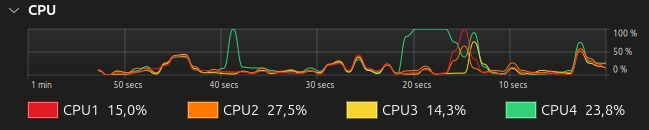
\includegraphics[width=0.8\textwidth]{./Imágenes/S1_SystemMonitor.jpg}
    \caption{Monitorización de la ejecución del programa.}
    \label{fig:monitorizacion}
\end{figure}